%%%%%%%%%%%%%%%%%%%%%%%%%%%%%%%%%%%%%%%%%
% University Assignment Title Page 
% LaTeX Template
% Version 1.0 (27/12/12)
%
% This template has been downloaded from:
% http://www.LaTeXTemplates.com
%
% Original author:
% WikiBooks (http://en.wikibooks.org/wiki/LaTeX/Title_Creation)
%
% License:
% CC BY-NC-SA 3.0 (http://creativecommons.org/licenses/by-nc-sa/3.0/)
% 
% Instructions for using this template:
% This title page is capable of being compiled as is. This is not useful for 
% including it in another document. To do this, you have two options: 
%
% 1) Copy/paste everything between \begin{document} and \end{document} 
% starting at \begin{titlepage} and paste this into another LaTeX file where you 
% want your title page.
% OR
% 2) Remove everything outside the \begin{titlepage} and \end{titlepage} and 
% move this file to the same directory as the LaTeX file you wish to add it to. 
% Then add \input{./title_page_1.tex} to your LaTeX file where you want your
% title page.
%
%%%%%%%%%%%%%%%%%%%%%%%%%%%%%%%%%%%%%%%%%
%\title{Title page with logo}
%----------------------------------------------------------------------------------------
%	PACKAGES AND OTHER DOCUMENT CONFIGURATIONS
%----------------------------------------------------------------------------------------

\documentclass[11pt, a4paper]{article}

\usepackage[utf8x]{inputenc}
\usepackage[spanish, es-tabla, es-nodecimaldot]{babel}
\addto\captionsspanish{\renewcommand{\contentsname}{Contenido}}

\usepackage{graphicx}
\usepackage{amsmath}
\usepackage[table,xcdraw]{xcolor}

\usepackage[a4paper, 					% Page Layout
                     %showframe,				% This shows the frame
                     twoside, includehead,
                     footskip=7mm, headsep=6mm, headheight=4.8mm,
                     marginparsep=2mm, marginparwidth=22mm,
                     top=25mm, bottom=25mm, inner=30mm, outer=25mm]{geometry}

\usepackage[colorinlistoftodos]{todonotes}
\usepackage{siunitx}
\usepackage{lipsum}
\usepackage{setspace}
\usepackage{caption}
\usepackage{physics}
\usepackage{tikz}
\usetikzlibrary{babel}	
\usetikzlibrary{matrix,calc}
\captionsetup[table]{position=bottom}   %% or below
\makeatletter
\newcommand{\mypm}{\mathbin{\mathpalette\@mypm\relax}}
\newcommand{\@mypm}[2]{\ooalign{%
  \raisebox{.1\height}{$#1+$}\cr
  \smash{\raisebox{-.6\height}{$#1-$}}\cr}}
\makeatother
\usepackage{lscape}
\usepackage{float}
\newcommand\tab[1][1cm]{\hspace*{#1}}

\begin{document}

\begin{titlepage}

\newcommand{\HRule}{\rule{\linewidth}{0.5mm}} % Defines a new command for the horizontal lines, change thickness here

\center % Center everything on the page
 
%----------------------------------------------------------------------------------------
%	HEADING SECTIONS
%----------------------------------------------------------------------------------------

\textsc{\LARGE  Instituto Tecnológico de Buenos Aires}\\[1.5cm] % Name of your university/college
\textsc{\large Electrónica III}\\[0.5cm] % Minor heading such as course title

%----------------------------------------------------------------------------------------
%	TITLE SECTION
%----------------------------------------------------------------------------------------

\HRule \\[0.4cm]
{ \huge \bfseries Trabajo Práctico N°1}\\[0.4cm] % Title of your document
\HRule \\[1.5cm]
 \textsc{\large Grupo 2}\\[0.5cm] 
%----------------------------------------------------------------------------------------
%	AUTHOR SECTION
%----------------------------------------------------------------------------------------

\begin{minipage}{0.5\textwidth}
\begin{flushleft} \large
\emph{Integrantes:}\\
Santiago \textsc{Arribere, 59169} \newline % Your name
Gonzalo \textsc{Davidov, 59117}\newline
R. Nicolás \textsc{Trozzo, 59434}\newline
Matías \textsc{Francois, 59828}\newline
Pablo \textsc{Scheinfeld, 59065}

\end{flushleft}
\end{minipage}
~
\begin{minipage}{0.4\textwidth}
\begin{flushright} \large
\emph{Profesores:} \\
Kevin \textsc{Dewald}\\ % Supervisor's Name
Pablo Enrique \textsc{Wundes}\\
Miguel Pablo \textsc{Aguirre}
\end{flushright}
\end{minipage}\\[1cm]

% If you don't want a supervisor, uncomment the two lines below and remove the section above
%\Large \emph{Author:}\\
%John \textsc{Smith}\\[3cm] % Your name

%----------------------------------------------------------------------------------------
%	DATE SECTION
%----------------------------------------------------------------------------------------

{\large 4 de septiembre de 2019}\\[1cm] % Date, change the \today to a set date if you want to be precise

%----------------------------------------------------------------------------------------
%	LOGO SECTION
%----------------------------------------------------------------------------------------
\vspace{5cm}
%
\includegraphics[scale=0.2]{images/caratula/logo2.png}\\[1cm] % Include a department/university logo - this will require the graphicx package
\begin{center}
    \begin{table}[H]
        \begin{tabular}{p{165mm}}
        \hline
        
\textit{Abstract}\\
El presente informe tiene como objetivo trabajar sobre diferentes conceptos relacionados con la electr\'onica digital, 
tales como la l\'ogica combinacional y el \'algebra booleana, para as\'i poder aplicar lo aprendido en los ejercicios planteados por la c\'atedra.
A partir de estos conceptos se analizan los diversos casos de circuitos l\'ogicos para su posterior implementaci\'on en el lenguaje Verilog. 
De esta manera la persona que lea este informe podr\'a familiarizarse con la resoluci\'on de circuitos  


 \\ \hline
        \end{tabular}
    \end{table}
\end{center}
%----------------------------------------------------------------------------------------

\vfill % Fill the rest of the page with whitespace

\end{titlepage}

\tableofcontents
\newpage
\newpage
\section{Ejercicio 1}
\subsection{An\'alisis}
\noindent
Este ejercicio consiste en implementar un programa el cual dada cierta convenci\'on de punto fijo devuelva el rango y la resoluci\'on del mismo.\\
La convenci\'on se recibe al momento de ejecutar el programa en el siguiente orden: Signado, Bits parte entera y Bits parte fraccionaria, a lo largo del presente informe se har\'a referencia a los mismos como: 's', 'a' y 'b' respectivamente.\\
Inicialmente para el c\'alculo de la resoluci\'on se puede observar que la misma viene dada por el bit menos significativo, por lo tanto responde a la expresi\'on \ref{eqn:resolucion}, no importando si se est\'a trabajando con un n\'umero signado o no signado.
\begin{equation}
    Res = 2^{-b}
    \label{eqn:resolucion}
\end{equation}
Luego para hallar el rango se calcula la diferencia entre el mayor n\'umero que es posible representar y el menor, de esta forma se obtienen las expresiones \ref{eqn:ran_no_sig} y \ref{eqn:ran_sig}, para n\'umeros signados y no signados, respectivamente. Con esto se puede evidenciar que el rango tampoco depende de la convenci\'on de signo que se proponga utilizar, por lo tanto 's' solo debe ser validado para el correcto funcionamiento del programa.
\begin{equation}
    Ran = (Max-Min) = \sum_{i=-b}^{a-1}2^{i} - 0 = \sum_{i=-b}^{a-1}2^{i} 
    \label{eqn:ran_no_sig}
\end{equation}
\begin{equation}
    Ran = (Max-Min) = \sum_{i=-b}^{a-2}2^{i} - (-2^{a-1}) = \sum_{i=-b}^{a-1}2^{i} 
    \label{eqn:ran_sig}
\end{equation}
\subsection{Elecci\'on del lenguaje}
\noindent
Inicialmente, al ser un programa aparentemente sencillo, se hab\'ia optado por utilizar el lenguaje 'C', de esta forma se procedi\'o a realizar el algoritmo necesario para la validaci\'on, el mismo comprueba que 's' sea '1' o '0', e inicialmente se comprob\'o solamente que 'a' y 'b' fuesen n\'umeros enteros, y que ambos sean distintos de '0' simultáneamente. Luego de la validaci\'on de datos, se desarroll\'o el algoritmo del calculo del rango y la resoluci\'on, pero al momento de tener que imprimir la respuesta en pantalla no se pudo obtener el formato deseado debido a la forma de representar n\'umeros con decimales, debido a que el lenguaje no ajusta din\'amicamente la forma de representar este tipo de números, sino que en lugar de eso muestra una cantidad especificada de cifras significativas del valor.\\
Por lo tanto para poder solucionar esta limitaci\'on de decidi\'o cambiar al lenguaje 'C++', con el cual la forma de representar en pantalla los n\'umeros era la requerida para responder con lo solicitado.\\
Otra limitaci\'on que se encontró durante la resolución de este apartado fue el l\'imite num\'erico que era posible procesar, ya que, al utilizar el tipo de dato \textit{float}, la resoluci\'on propia del mismo es de $2^{-126}$, por lo tanto 'b'=126 es el l\'imite superior que el programa puede recibir como valor para la parte fraccionaria.\\
Y como limitación para la parte entera se tiene 'a'=24, ya que para valores mayores del mismo, la precisión del n\'umero representado deja de ser exacta y comienza a tomar aproximaciones a n\'umeros múltiplos de potencias de 2.\\ 
\newpage
\newpage
\section{Ejercicio 2}
\noindent
El ejercicio 2 se basa resolver dos problemas, el primero, un ejercicio de 5 variables, dado en funci\'on de mint\'erminos y el segundo, de 4 variables, en funci\'on de maxt\'erminos.\par
\subsection{Primera parte}

\begin{displaymath}
f(A,B,C,D,E) = \sum{m(0,2,4,7,8,10,12,16,18,20,23,24,25,26,27,28)}\par
\end{displaymath}
\subsubsection{Resoluci\'on mediante algebra booleana}
\vspace{5mm}
\noindent
La expresi\'on obtenida por los minterminos dados es la siguiente:\\

$f(a,b,c,d,e) =  \overline{a}.\overline{b}.\overline{c}.\overline{d}.\overline{e} + \overline{a}.\overline{b}.\overline{c}.d.\overline{e} +
\vspace{5mm}\overline{a}.\overline{b}.c.\overline{d}.\overline{e} + \overline{a}.\overline{b}.c.d.e + \overline{a}.b.\overline{c}.\overline{d}.\overline{e} + \overline{a}.b.\overline{c}.d.\overline{e} + \vspace{5mm}\overline{a}.b.c.\overline{d}.\overline{e} + a.\overline{b}.\overline{c}.\overline{d}.\overline{e} + a.\overline{b}.\overline{c}.d.\overline{e} + a.\overline{b}.c.\overline{d}.\overline{e} + a.\overline{b}.c.d.e + a.b.\overline{c}.\overline{d}.\overline{e} + a.b.\overline{c}.\overline{d}.e + a.b.\overline{c}.d.\overline{e} + a.b.\overline{c}.d.e + a.b.c.\overline{d}.\overline{e} $
\vspace{5mm}

\noindent
Se puede ampliar la expresi\'on, con la finalidad de luego reducirla significativamente a partir de las simplificaci\'ones del \'algebra booleana :\\

$f(a,b,c,d,e) =  \overline{a}.\overline{b}.\overline{c}.\overline{d}.\overline{e} + \overline{a}.\overline{b}.\overline{c}.d.\overline{e} +
\vspace{5mm}\overline{a}.\overline{b}.c.\overline{d}.\overline{e} + \overline{a}.\overline{b}.c.d.e + \overline{a}.b.\overline{c}.\overline{d}.\overline{e} + \overline{a}.b.\overline{c}.d.\overline{e} + \vspace{5mm}\overline{a}.b.c.\overline{d}.\overline{e} + a.\overline{b}.\overline{c}.\overline{d}.\overline{e} + a.\overline{b}.\overline{c}.d.\overline{e} + a.\overline{b}.c.\overline{d}.\overline{e} + a.\overline{b}.c.d.e + a.b.\overline{c}.\overline{d}.\overline{e} + a.b.\overline{c}.\overline{d}.e + a.b.\overline{c}.d.\overline{e} + \vspace{5mm}a.b.\overline{c}.d.e + a.b.c.\overline{d}.\overline{e} + \textcolor{red}{a.\overline{b}.\overline{c}.\overline{d}.\overline{e}} \color{black}+
\textcolor{red}{a.b.\overline{c}.\overline{d}.\overline{e}} \color{black}+\textcolor{red}{ \overline{a}.\overline{b}.\overline{c}.\overline{d}.\overline{e}}\textcolor{black}{+} \textcolor{red}{a.b.\overline{c}.d.\overline{e}} \color{black}+ \textcolor{red}{\overline{a}.b.\overline{c}.\overline{d}.\overline{e}} \color{black}{+} \textcolor{red}{a.b.\overline{c}.\overline{d}.\overline{e}}$
\vspace{5mm}\par

\noindent
De aqu\'i utilizando la propiedad de absorci\'on \par
\vspace{5mm}

$f(a,b,c,d,e) =  \color{red}{\overline{a}.\overline{b}.\overline{c}.\overline{d}.\overline{e}} \color{black}+ \overline{a}.\overline{b}.\overline{c}.d.\overline{e} \color{black}+
\vspace{5mm}\color{green}{\overline{a}.\overline{b}.c.\overline{d}.\overline{e}} \color{black}+ \color{blue}{\overline{a}.\overline{b}.c.d.e} \color{black}\color{black}+ \color{yellow}{\overline{a}.b.\overline{c}.\overline{d}.\overline{e}} \color{black}+ \color{pink}{\overline{a}.b.\overline{c}.d.\overline{e}} \color{black}+ \vspace{5mm}\color{violet}{\overline{a}.b.c.\overline{d}.\overline{e}} \color{black}+ \color{brown}{a.\overline{b}.\overline{c}.\overline{d}.\overline{e}} \color{black}+ a.\overline{b}.\overline{c}.d.\overline{e} \color{black}+ \color{orange}{a.\overline{b}.c.\overline{d}.\overline{e}} \color{black}+ \color{blue}{a.\overline{b}.c.d.e} \color{black}+ \color{yellow}{a.b.\overline{c}.\overline{d}.\overline{e}} \color{black}+ \color{gray}{a.b.\overline{c}.\overline{d}.e} \color{black}+ \color{cyan}{a.b.\overline{c}.d.\overline{e}} \color{black}+ \color{gray}{a.b.\overline{c}.d.e} \color{black}+ \vspace{5mm}\color{orange}{a.b.c.\overline{d}.\overline{e}} \color{black}+ \color{magenta}{a.\overline{b}.\overline{c}.\overline{d}.\overline{e}} \color{black}+
a.b.\overline{c}.\overline{d}.\overline{e} \color{black}+ \color{green}{\overline{a}.\overline{b}.\overline{c}.\overline{d}.\overline{e}} \color{black}+ \color{pink}{a.b.\overline{c}.d.\overline{e}} \color{black}+ \color{violet}{\overline{a}.b.\overline{c}.\overline{d}.\overline{e}} \color{black}+ \color{cyan}{a.b.\overline{c}.\overline{d}.\overline{e}}$
\vspace{8mm}\par
$
\color{black}{f(a,b,c,d,e) =}  \color{red}{\overline{a}.\overline{b}.\overline{c}.\overline{e}} \color{black}+
\vspace{5mm}\color{green}{\overline{a}.\overline{b}.\overline{d}.\overline{e}} \color{black}+ \color{blue}{\overline{b}.c.d.e} \color{black}+ \color{yellow}{b.\overline{c}.\overline{d}.\overline{e}} \color{black}+ \color{pink}{b.\overline{c}.d.\overline{e}} \color{black}+ \color{violet}{\overline{a}.b.\overline{d}.\overline{e}} \color{black}+ \color{brown}{a.\overline{b}.\overline{c}.\overline{e}} \color{black}+ \color{orange}{a.c.\overline{d}.\overline{e}} \color{black}+ \color{gray}{a.b.\overline{c}.e} \color{black}+ \color{cyan}{a.b.\overline{c}.\overline{e}} \color{black}+ \color{magenta}{a.\overline{c}.\overline{d}.\overline{e}}$
\vspace{8mm}\par

\noindent
Asi llegamos a:\vspace{8mm}\par

$
\color{black}{f(a,b,c,d,e) =}  \overline{a}.\overline{b}.\overline{c}.\overline{e} \color{black}+
\vspace{5mm}\overline{a}.\overline{b}.\overline{d}.\overline{e} \color{black}+ \overline{b}.c.d.e \color{black}+ b.\overline{c}.\overline{d}.\overline{e} \color{black}+ b.\overline{c}.d.\overline{e} \color{black}+ \overline{a}.b.\overline{d}.\overline{e} \color{black}+ a.\overline{b}.\overline{c}.\overline{e} \color{black}+ a.c.\overline{d}.\overline{e} \color{black}+ a.b.\overline{c}.e \color{black}+ a.b.\overline{c}.\overline{e} \color{black}+ a.\overline{c}.\overline{c}.\overline{e}$
\vspace{8mm}\par

\noindent
Luego de esto, nuevamente aplicaremos absorcion de la siguiente manera:\vspace{8mm}\par

$
\color{black}{f(a,b,c,d,e) =}  \color{red}{\overline{a}.\overline{b}.\overline{c}.\overline{e}} \color{black}+
\vspace{5mm}\color{green}{\overline{a}.\overline{b}.\overline{d}.\overline{e}} \color{black}+ \color{black}{\overline{b}.c.d.e} \color{black}+ \color{blue}{b.\overline{c}.\overline{d}.\overline{e} \color{black}+ b.\overline{c}.d.\overline{e}} \color{black}+ \color{green}{\overline{a}.b.\overline{d}.\overline{e}} \color{black}+ \color{red}{a.\overline{b}.\overline{c}.\overline{e}} \color{black}+ \color{magenta}{a.c.\overline{d}.\overline{e}} \color{black}+ \color{cyan}{a.b.\overline{c}.e + a.b.\overline{c}.\overline{e}} \color{black}+ \color{magenta}{a.\overline{c}.\overline{d}.\overline{e}}$
\vspace{8mm}\par
$
\color{black}{f(a,b,c,d,e) =}  \color{red}{\overline{b}.\overline{c}.\overline{e}} \color{black}+ \color{green}{\overline{a}.\overline{d}.\overline{e}} \color{black}+ \color{black}{\overline{b}.c.d.e} \color{black}+ \color{blue}{b.\overline{c}.\overline{e}} \color{black}+ \color{magenta}{a.\overline{d}.\overline{e}} \color{black}+ \color{cyan}{a.b.\overline{c}}$
\vspace{8mm}\par

Entonces hallamos la siguiente expresion:\vspace{8mm}\par

$
\color{black}{f(a,b,c,d,e) =}  \overline{b}.\overline{c}.\overline{e} + \overline{a}.\overline{d}.\overline{e} + \overline{b}.c.d.e + b.\overline{c}.\overline{e} + a.\overline{d}.\overline{e} + a.b.\overline{c}$
\vspace{8mm}\par

Para luego realizar una ultima absorci\'on:\vspace{8mm}\par

$
\color{black}{f(a,b,c,d,e) =}  \color{red}{\overline{b}.\overline{c}.\overline{e}} \color{black}+ \color{blue}{\overline{a}.\overline{d}.\overline{e}} \color{black}+ \color{black}{\overline{b}.c.d.e} \color{black}+ \color{red}{b.\overline{c}.\overline{e}} \color{black}+ \color{blue}{a.\overline{d}.\overline{e}} \color{black}+ \color{black}{a.b.\overline{c}}$
\vspace{8mm}\par


$
\color{black}{f(a,b,c,d,e) =}  \color{red}{\overline{c}.\overline{e}} \color{black}+ \color{blue}{\overline{d}.\overline{e}}\color{black} + \color{black}{\overline{b}.c.d.e} +  \color{black}{a.b.\overline{c}}$
\vspace{8mm}\par


\noindent
\color{black}De esta manera se obtiene la expresi\'on deseada:\par\vspace{5mm}

$f(a,b,c,d,e) =  \overline{c}.\overline{e} + \overline{d}.\overline{e} + \overline{b}.c.d.e + a.b.\overline{c}$
\vspace{8mm}\par
\subsubsection{Resoluci\'on mediante mapas de Karnaugh}


\newcommand{\implicantsol}[3][0]{
    \draw[rounded corners=3pt, fill=#3, opacity=0.3] ($(#2.north west)+(135:#1)$) rectangle ($(#2.south east)+(-45:#1)$);
    }


%internal group
%#1 - Optional. Space between node and grouping line. Default=0
%#2 - top left node
%#3 - bottom right node
%#4 - filling color
\newcommand{\implicant}[4][0]{
    \draw[rounded corners=3pt, fill=#4, opacity=0.3] ($(#2.north west)+(135:#1)$) rectangle ($(#3.south east)+(-45:#1)$);
    }

%group lateral borders
%#1 - Optional. Space between node and grouping line. Default=0
%#2 - top left node
%#3 - bottom right node
%#4 - filling color
\newcommand{\implicantcostats}[4][0]{
    \draw[rounded corners=3pt, fill=#4, opacity=0.3] ($(rf.east |- #2.north)+(90:#1)$)-| ($(#2.east)+(0:#1)$) |- ($(rf.east |- #3.south)+(-90:#1)$);
    \draw[rounded corners=3pt, fill=#4, opacity=0.3] ($(cf.west |- #2.north)+(90:#1)$) -| ($(#3.west)+(180:#1)$) |- ($(cf.west |- #3.south)+(-90:#1)$);
}

%group top-bottom borders
%#1 - Optional. Space between node and grouping line. Default=0
%#2 - top left node
%#3 - bottom right node
%#4 - filling color
\newcommand{\implicantdaltbaix}[4][0]{
    \draw[rounded corners=3pt, fill=#4, opacity=0.3] ($(cf.south -| #2.west)+(180:#1)$) |- ($(#2.south)+(-90:#1)$) -| ($(cf.south -| #3.east)+(0:#1)$);
    \draw[rounded corners=3pt, fill=#4, opacity=0.3] ($(rf.north -| #2.west)+(180:#1)$) |- ($(#3.north)+(90:#1)$) -| ($(rf.north -| #3.east)+(0:#1)$);
}

%group corners
%#1 - Optional. Space between node and grouping line. Default=0
%#2 - filling color
\newcommand{\implicantcantons}[2][0]{
    \draw[rounded corners=3pt, opacity=.3] ($(rf.east |- 0.south)+(-90:#1)$) -| ($(0.east |- cf.south)+(0:#1)$);
    \draw[rounded corners=3pt, opacity=.3] ($(rf.east |- 8.north)+(90:#1)$) -| ($(8.east |- rf.north)+(0:#1)$);
    \draw[rounded corners=3pt, opacity=.3] ($(cf.west |- 2.south)+(-90:#1)$) -| ($(2.west |- cf.south)+(180:#1)$);
    \draw[rounded corners=3pt, opacity=.3] ($(cf.west |- 10.north)+(90:#1)$) -| ($(10.west |- rf.north)+(180:#1)$);
    \fill[rounded corners=3pt, fill=#2, opacity=.3] ($(rf.east |- 0.south)+(-90:#1)$) -|  ($(0.east |- cf.south)+(0:#1)$) [sharp corners] ($(rf.east |- 0.south)+(-90:#1)$) |-  ($(0.east |- cf.south)+(0:#1)$) ;
    \fill[rounded corners=3pt, fill=#2, opacity=.3] ($(rf.east |- 8.north)+(90:#1)$) -| ($(8.east |- rf.north)+(0:#1)$) [sharp corners] ($(rf.east |- 8.north)+(90:#1)$) |- ($(8.east |- rf.north)+(0:#1)$) ;
    \fill[rounded corners=3pt, fill=#2, opacity=.3] ($(cf.west |- 2.south)+(-90:#1)$) -| ($(2.west |- cf.south)+(180:#1)$) [sharp corners]($(cf.west |- 2.south)+(-90:#1)$) |- ($(2.west |- cf.south)+(180:#1)$) ;
    \fill[rounded corners=3pt, fill=#2, opacity=.3] ($(cf.west |- 10.north)+(90:#1)$) -| ($(10.west |- rf.north)+(180:#1)$) [sharp corners] ($(cf.west |- 10.north)+(90:#1)$) |- ($(10.west |- rf.north)+(180:#1)$) ;
}

%Empty Karnaugh map 4x4
\newenvironment{Karnaugh}%
{
\begin{tikzpicture}[baseline=(current bounding box.north),scale=0.8]
\draw (0,0) grid (4,4);
\draw (0,4) -- node [pos=0.7,above right,anchor=south west] {bc} node [pos=0.7,below left,anchor=north east] {de} ++(135:1);
%
\matrix (mapa) [matrix of nodes,
        column sep={0.8cm,between origins},
        row sep={0.8cm,between origins},
        every node/.style={minimum size=0.3mm},
        anchor=8.center,
        ampersand replacement=\&] at (0.5,0.5)
{
                       \& |(c00)| 00         \& |(c01)| 01         \& |(c11)| 11         \& |(c10)| 10         \& |(cf)| \phantom{00} \\
|(r00)| 00             \& |(0)|  \phantom{0} \& |(1)|  \phantom{0} \& |(3)|  \phantom{0} \& |(2)|  \phantom{0} \&                     \\
|(r01)| 01             \& |(4)|  \phantom{0} \& |(5)|  \phantom{0} \& |(7)|  \phantom{0} \& |(6)|  \phantom{0} \&                     \\
|(r11)| 11             \& |(12)| \phantom{0} \& |(13)| \phantom{0} \& |(15)| \phantom{0} \& |(14)| \phantom{0} \&                     \\
|(r10)| 10             \& |(8)|  \phantom{0} \& |(9)|  \phantom{0} \& |(11)| \phantom{0} \& |(10)| \phantom{0} \&                     \\
|(rf) | \phantom{00}   \&                    \&                    \&                    \&                    \&                     \\
};
}%
{
\end{tikzpicture}
}

%Empty Karnaugh map 2x4
\newenvironment{Karnaughvuit}%
{
\begin{tikzpicture}[baseline=(current bounding box.north),scale=0.8]
\draw (0,0) grid (4,2);
\draw (0,2) -- node [pos=0.7,above right,anchor=south west] {eb} node [pos=0.7,below left,anchor=north east] {b} ++(135:1);
%
\matrix (mapa) [matrix of nodes,
        column sep={0.8cm,between origins},
        row sep={0.8cm,between origins},
        every node/.style={minimum size=0.3mm},
        anchor=4.center,
        ampersand replacement=\&] at (0.5,0.5)
{
                      \& |(c00)| 00         \& |(c01)| 01         \& |(c11)| 11         \& |(c10)| 10         \& |(cf)| \phantom{00} \\
|(r00)| 0             \& |(0)|  \phantom{0} \& |(1)|  \phantom{0} \& |(3)|  \phantom{0} \& |(2)|  \phantom{0} \&                     \\
|(r01)| 1             \& |(4)|  \phantom{0} \& |(5)|  \phantom{0} \& |(7)|  \phantom{0} \& |(6)|  \phantom{0} \&                     \\
|(rf) | \phantom{00}  \&                    \&                    \&                    \&                    \&                     \\
};
}%
{
\end{tikzpicture}
}

%Empty Karnaugh map 2x2
\newenvironment{Karnaughquatre}%
{
\begin{tikzpicture}[baseline=(current bounding box.north),scale=0.8]
\draw (0,0) grid (2,2);
\draw (0,2) -- node [pos=0.7,above right,anchor=south west] {e} node [pos=0.7,below left,anchor=north east] {b} ++(135:1);
%
\matrix (mapa) [matrix of nodes,
        column sep={0.8cm,between origins},
        row sep={0.8cm,between origins},
        every node/.style={minimum size=0.3mm},
        anchor=2.center,
        ampersand replacement=\&] at (0.5,0.5)
{
          \& |(c00)| 0          \& |(c01)| 1  \\
|(r00)| 0 \& |(0)|  \phantom{0} \& |(1)|  \phantom{0} \\
|(r01)| 1 \& |(2)|  \phantom{0} \& |(3)|  \phantom{0} \\
};
}%
{
\end{tikzpicture}
}

%Defines 8 or 16 values (0,1,X)
\newcommand{\contingut}[1]{%
\foreach \x [count=\xi from 0]  in {#1}
     \path (\xi) node {\x};
}

%Places 1 in listed positions
\newcommand{\minterms}[1]{%
    \foreach \x in {#1}
        \path (\x) node {1};
}

%Places 0 in listed positions
\newcommand{\maxterms}[1]{%
    \foreach \x in {#1}
        \path (\x) node {0};
}

%Places X in listed positions
\newcommand{\indeterminats}[1]{%
    \foreach \x in {#1}
        \path (\x) node {X};
}

\tab[1.5cm] a = 0 \tab[4cm] a = 1\newline
\begin{Karnaugh}
    \minterms{0,1,2,3,8,10,13}
    \maxterms{4,5,6,7,9,11,12,14,15}
    \implicant{0}{2}{red}
    \implicantcantons[2pt]{blue}
    \implicantsol{13}{green}
\end{Karnaugh}
%
\begin{Karnaugh}
    \minterms{0,1,2,3,6,8,10,13,14}
    \maxterms{4,5,7,9,11,12,15}
    \implicant{0}{2}{red}
    \implicantcantons[2pt]{blue}
    \implicantsol{13}{green}
    \implicantdaltbaix[3pt]{10}{2}{yellow}
\end{Karnaugh}
\par
\noindent
De aqu\'i, mediante la separaci\'on por grupos marcada previamente en los mapas de Karnaugh, se observa de que variables depende cada grupo y si estas estan negadas o no, llegando a la siguiente expresi\'on: \par\vspace{5mm}

$f(A,B,C,D,E)$ =  \overline{C}.\overline{E} + \overline{D}.\overline{E} + \overline{B}.C.D.E + A.B.\overline{C}
\vspace{8mm}\par
\noindent
Como era de esperarse, el resultado obtenido mediante mapas de Karnaugh es igual a la simplificaci\'on obtenida mediante algebra booleana.
\subsubsection{Representaci\'on con compuertas AND, OR y NOT}
\noindent
La representaci\'on de la expresion obtenida previamente mediante compuertas logicas AND, OR y NOT se puede ver a continuaci\'on.

\begin{figure}[h!]
    \centering
    \begin{minipage}{0.85\textwidth}
        \centering
        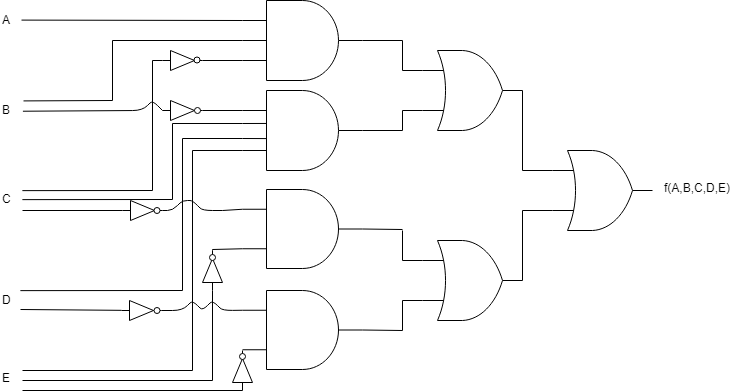
\includegraphics[width=0.9\textwidth]{images/ej2/ej2andornot.png} % first figure itself
         \label{fig:ej2andornot}
    \end{minipage}\hfill
\end{figure}

\subsubsection{Representaci\'on con compuertas NAND}
\noindent
La representaci\'on de la expresi\'on encontrada previamente mediante compuertas logicas NAND se puede ver a continuaci\'on.

\begin{figure}[H]
    \centering
    \begin{minipage}{0.85\textwidth}
        \centering
        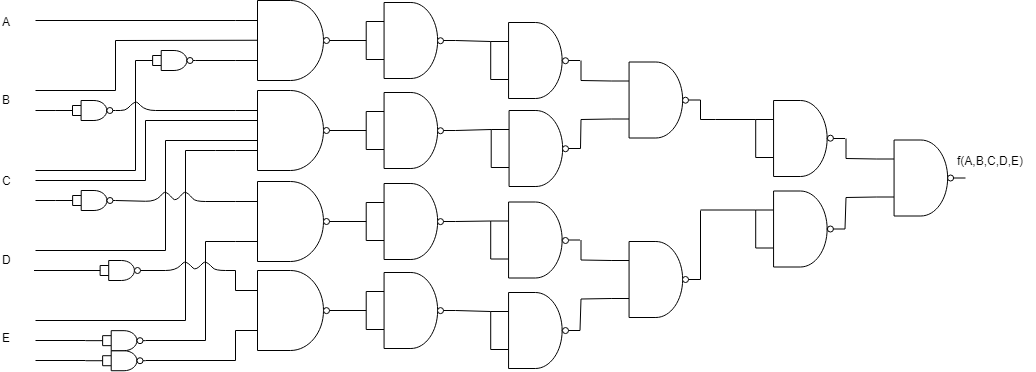
\includegraphics[width=0.9\textwidth]{images/ej2/ej2nand.png} % first figure itself
         \label{fig:ej2nand}
    \end{minipage}\hfill
\end{figure}

%%parte B

\subsection{Segunda parte}

\begin{displaymath}
f(d,c,b,a) = \prod{(M0,M2,M4,M7,M8,M10,M12)}
\end{displaymath}

\subsubsection{Resoluci\'on mediante algebra booleana}
\vspace{5mm}
\noindent
La expresi\'on obtenida por los maxt\'erminos dados es la siguiente:\\


$f(d,c,b,a)=(d+c+b+a)\cdot(d+c+\overline{b}+a)\cdot(d+\overline{c}+b+a)\cdot(d+\overline{c}+\overline{b}+\overline{a})\cdot(\overline{d}+c+b+a)\cdot(\overline{d}+c+\overline{b}+a)\cdot(\overline{d}+\overline{c}+b+a) $
\vspace{5mm}


\noindent
De aqu\'i utilizando la propiedad de absorci\'on podremos reducir la expresi\'on a:\par
\vspace{5mm}

$f(d,c,b,a)=\color{red}{(d+c+b+a)}\color{black}\cdot\color{red}{(d+c+\overline{b}+a)}\color{black}\cdot\color{blue}{(d+\overline{c}+b+a)}\color{black}\cdot\color{black}{(d+\overline{c}+\overline{b}+\overline{a})}\color{black}\cdot\color{green}{(\overline{d}+c+b+a)}\color{black}\cdot\color{green}{(\overline{d}+c+\overline{b}+a)}\color{black}\cdot\color{blue}{(\overline{d}+\overline{c}+b+a)}$
\vspace{8mm}\par
$f(d,c,b,a)=\color{red}{(d+c+a)}\color{black}\cdot\color{blue}{(\overline{c}+b+a)}\color{black}\cdot\color{black}{(d+\overline{c}+\overline{b}+\overline{a})}\color{black}\cdot\color{green}{(\overline{d}+c+a)}$
\vspace{8mm}\par

\noindent
De esta forma, aprovechando el hecho de que x.x=x lo que haremos ser\'a traer los t\'erminos: $(d+c+b+a) y (\overline{d}+c+b+a)$ de la primer linea de donde partimos como productos, de esta forma obtendremos la siguiente expresi\'on:\par
\vspace{5mm}

$f(d,c,b,a)={(d+c+a)}\cdot{(\overline{c}+b+a)}\cdot{(d+\overline{c}+\overline{b}+\overline{a})}\cdot{(\overline{d}+c+a)}\cdot{(d+c+b+a)}\cdot{(\overline{d}+c+b+a)}$
\vspace{8mm}\par

\noindent
Ahora utilizando nuevamiente la propiedad de absorci\'on tendremos:\par
\vspace{5mm}

$f(d,c,b,a)=\color{red}{(d+c+a)}\color{black}\cdot{(\overline{c}+b+a)}\cdot{(d+\overline{c}+\overline{b}+\overline{a})}\cdot\color{red}{(\overline{d}+c+a)}\color{black}\cdot\color{blue}{(d+c+b+a)}\color{black}\cdot\color{blue}{(\overline{d}+c+b+a)}$
\vspace{8mm}\par

$f(d,c,b,a)=\color{red}{(c+a)}\color{black}\cdot{(\overline{c}+b+a)}\cdot{(d+\overline{c}+\overline{b}+\overline{a})}\cdot\color{blue}{(c+b+a)}$
\vspace{8mm}\par

\noindent
\color{black}Nuevamente realizamos una \'ultima absorci\'on:\par\vspace{5mm}

$f(d,c,b,a)=\color{black}{(c+a)}\color{black}\cdot\color{red}{(\overline{c}+b+a)}\color{black}\cdot{(d+\overline{c}+\overline{b}+\overline{a})}\cdot\color{red}{(c+b+a)}$
\vspace{8mm}\par


$f(d,c,b,a)=\color{black}{(c+a)}\color{black}\cdot\color{red}{(b+a)}\color{black}\cdot{(d+\overline{c}+\overline{b}+\overline{a})}$
\vspace{8mm}\par


\noindent
\color{black}Finalmente, la expresi\'on hallada es:\par\vspace{5mm}

$f(d,c,b,a)=\color{black}{(c+a)}\cdot{(b+a)}\cdot{(d+\overline{c}+\overline{b}+\overline{a})}$
\vspace{8mm}\par
\subsubsection{Resoluci\'on mediante mapas de Karnaugh}


%Empty Karnaugh map 4x4
\newenvironment{Karnaugh2}%
{
\begin{tikzpicture}[baseline=(current bounding box.north),scale=0.8]
\draw (0,0) grid (4,4);
\draw (0,4) -- node [pos=0.7,above right,anchor=south west] {dc} node [pos=0.7,below left,anchor=north east] {ba} ++(135:1);
%
\matrix (mapa) [matrix of nodes,
        column sep={0.8cm,between origins},
        row sep={0.8cm,between origins},
        every node/.style={minimum size=0.3mm},
        anchor=8.center,
        ampersand replacement=\&] at (0.5,0.5)
{
                       \& |(c00)| 00         \& |(c01)| 01         \& |(c11)| 11         \& |(c10)| 10         \& |(cf)| \phantom{00} \\
|(r00)| 00             \& |(0)|  \phantom{0} \& |(1)|  \phantom{0} \& |(3)|  \phantom{0} \& |(2)|  \phantom{0} \&                     \\
|(r01)| 01             \& |(4)|  \phantom{0} \& |(5)|  \phantom{0} \& |(7)|  \phantom{0} \& |(6)|  \phantom{0} \&                     \\
|(r11)| 11             \& |(12)| \phantom{0} \& |(13)| \phantom{0} \& |(15)| \phantom{0} \& |(14)| \phantom{0} \&                     \\
|(r10)| 10             \& |(8)|  \phantom{0} \& |(9)|  \phantom{0} \& |(11)| \phantom{0} \& |(10)| \phantom{0} \&                     \\
|(rf) | \phantom{00}   \&                    \&                    \&                    \&                    \&                     \\
};
}%
{
\end{tikzpicture}
}



\begin{center}
\begin{Karnaugh2}
    \minterms{4,5,6,7,9,11,12,14,15}
    \maxterms{0,1,8,3,2,13,10}
    \implicant{0}{2}{red}
    \implicantcantons[2pt]{blue}
    \implicantsol{13}{green}
\end{Karnaugh2}
\end{center}
\par
\noindent
De aqu\'i, mediante la separaci\'on por grupos marcada previamente en los mapas de Karnaugh, se observa de cuales variables depende cada grupo y si estas est\'an negadas o no, llegando a la siguiente expresi\'on: \par\vspace{5mm}

$f(d,c,b,a)=\color{black}{(c+a)}\cdot{(b+a)}\cdot{(d+\overline{c}+\overline{b}+\overline{a})}$
\vspace{8mm}\par
\noindent
Como era de esperarse, el resultado obtenido mediante mapas de Karnaugh es igual a la simplificaci\'on obtenida mediante algebra booleana.
\subsubsection{Representaci\'on con compuertas AND, OR y NOT}
\noindent
La representaci\'on de la expresi\'on obtenida previamente mediante compuertas l\'ogicas AND, OR y NOT se puede ver a continuaci\'on, en la figura \ref{fig:ej2b}

\begin{figure}[H]
    \centering
    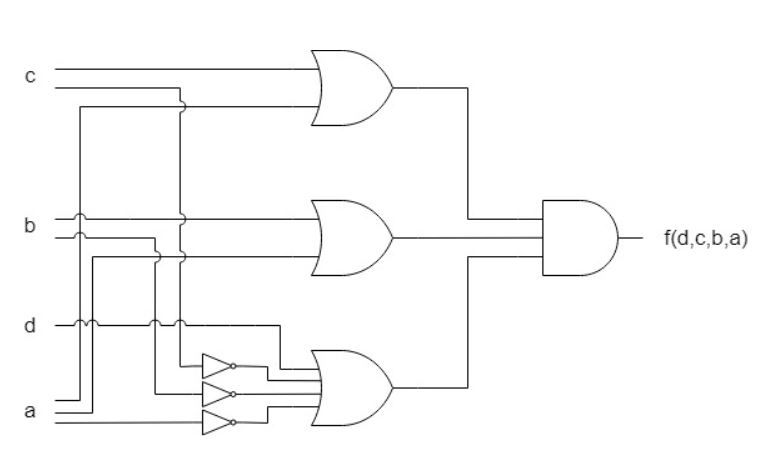
\includegraphics[scale=0.55]{images/ej2/circuito1_ej2_parteb.JPG}
    \caption{Circuito con compuertas AND, OR y NOT}
    \label{fig:ej2b}
\end{figure}

\subsubsection{Representaci\'on con compuertas NAND}
\noindent
La representaci\'on de la expresi\'on obtenida previamente mediante compuertas l\'ogicas NAND se puede ver a continuaci\'on en la figura \ref{fig:ej2bnand}

\begin{figure}[H]
    \centering
    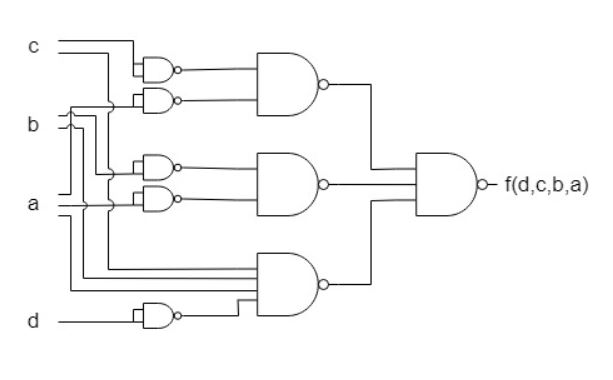
\includegraphics[scale=0.7]{images/ej2/circuito2_ej2_parteb.JPG}
    \caption{Circuito con compuertas NAND}
    \label{fig:ej2bnand}
\end{figure}\\
\newpage
\newpage
\section{Ejercicio 3}
\noindent
El ejercicio consta en crear mediante el uso del lenguaje Verilog un encoder de cuatro entradas y dos salidas y un demux de cuatro salidas con dos \textit{select lines}.\par
Se tiene como consideración que ante cualquier entrada no esperada la salida será alta impedancia, es decir, Z.\newline
A continuaci\'on se muestran las tablas de verdad:

\begin{table}[H]
    \center
    \begin{tabular}{|lll|llll|}
    \hline
    \textbf{S1} & \textbf{S2} & \textbf{In} & \textbf{Out0} & \textbf{Out1} & \textbf{Out2} & \textbf{Out3} \\ \hline
    0           & 0           & 0           & 0             & 0             & 0             & 0             \\
    0           & 0           & 1           & 0             & 0             & 0             & 1             \\
    0           & 1           & 0           & 0             & 0             & 0             & 0             \\
    0           & 1           & 1           & 0             & 0             & 1             & 0             \\
    1           & 0           & 0           & 0             & 0             & 0             & 0             \\
    1           & 0           & 1           & 0             & 1             & 0             & 0             \\
    1           & 1           & 0           & 0             & 0             & 0             & 0             \\
    1           & 1           & 1           & 1             & 0             & 0             & 0             \\ \hline
    \end{tabular}
    \caption{Tabla de verdad de el demux de 4 salidas}
    \end{table}

    \begin{table}[H]
        \center
        \begin{tabular}{|cccc|cc|}
        \hline
        \multicolumn{1}{|l}{\textbf{In1}} & \multicolumn{1}{l}{\textbf{In2}} & \multicolumn{1}{l}{\textbf{In3}} & \multicolumn{1}{l|}{\textbf{In4}} & \multicolumn{1}{l}{\textbf{Out0}} & \multicolumn{1}{l|}{\textbf{Out1}} \\ \hline
        1                                 & 0                                & 0                                & 0                                 & 0                                 & 0                                  \\
        0                                 & 1                                & 0                                & 0                                 & 0                                 & 1                                  \\
        0                                 & 0                                & 1                                & 0                                 & 1                                 & 0                                  \\
        0                                 & 0                                & 0                                & 1                                 & 1                                 & 1                                  \\ \hline
        \end{tabular}
        \caption{Tabla de verdad de el encoder de 4 entradas}
        \end{table}
\newpage
\section{Ejercicio 4}
\subsection{Expresi\'on en funci\'on de los mint\'erminos}
\noindent
Con el fin de convertir un número binario de 4 bits en su equivalente en código de Gray, se plantearon todas las posibilidades en la siguiente tabla de verdad, donde $Y_0$, $Y_1$, $Y_2$ e $Y_3$ representan las correspondientes salidas y A, B, C y D las entradas del sistema. Ambas se encuentran mostradas en forma ordenada, tomando $Y_0$ como el bit m\'as significativo y $Y_3$ como el bit menos significativo. De la misma forma, para las entradas, A reprensenta el bit m\'as significativo y D el menos significativo.

\begin{table}[h!]
\centering
\begin{tabular}{|cccc|cccc|}
\hline

\multicolumn{1}{|c|}{A} & \multicolumn{1}{c|}{B}   & \multicolumn{1}{c|}{C}   & D                        & \multicolumn{1}{c|}{$Y_0$}   & \multicolumn{1}{c|}{$Y_1$}   & \multicolumn{1}{c|}{$Y_2$}   & $Y_3$                        \\ \hline
\rowcolor[HTML]{34FF34} 
0                       & 0                        & 0                        & 0                        & \cellcolor[HTML]{FD6864}0 & \cellcolor[HTML]{FD6864}0 & \cellcolor[HTML]{FD6864}0 & \cellcolor[HTML]{FD6864}0 \\
\rowcolor[HTML]{34FF34} 
0                       & 0                        & 0                        & 1                        & \cellcolor[HTML]{FD6864}0 & \cellcolor[HTML]{FD6864}0 & \cellcolor[HTML]{FD6864}0 & \cellcolor[HTML]{FD6864}1 \\
\rowcolor[HTML]{34FF34} 
0                       & 0                        & 1                        & 0                        & \cellcolor[HTML]{FD6864}0 & \cellcolor[HTML]{FD6864}0 & \cellcolor[HTML]{FD6864}1 & \cellcolor[HTML]{FD6864}1 \\
\rowcolor[HTML]{34FF34} 
0                       & {\color[HTML]{333333} 0} & {\color[HTML]{333333} 1} & {\color[HTML]{333333} 1} & \cellcolor[HTML]{FD6864}0 & \cellcolor[HTML]{FD6864}0 & \cellcolor[HTML]{FD6864}1 & \cellcolor[HTML]{FD6864}0 \\
\rowcolor[HTML]{34FF34} 
0                       & {\color[HTML]{333333} 1} & {\color[HTML]{333333} 0} & {\color[HTML]{333333} 0} & \cellcolor[HTML]{FD6864}0 & \cellcolor[HTML]{FD6864}1 & \cellcolor[HTML]{FD6864}1 & \cellcolor[HTML]{FD6864}0 \\
\rowcolor[HTML]{34FF34} 
0                       & {\color[HTML]{333333} 1} & {\color[HTML]{333333} 0} & {\color[HTML]{333333} 1} & \cellcolor[HTML]{FD6864}0 & \cellcolor[HTML]{FD6864}1 & \cellcolor[HTML]{FD6864}1 & \cellcolor[HTML]{FD6864}1 \\
\rowcolor[HTML]{34FF34} 
0                       & {\color[HTML]{333333} 1} & {\color[HTML]{333333} 1} & {\color[HTML]{333333} 0} & \cellcolor[HTML]{FD6864}0 & \cellcolor[HTML]{FD6864}1 & \cellcolor[HTML]{FD6864}0 & \cellcolor[HTML]{FD6864}1 \\
\rowcolor[HTML]{34FF34} 
0                       & {\color[HTML]{333333} 1} & {\color[HTML]{333333} 1} & {\color[HTML]{333333} 1} & \cellcolor[HTML]{FD6864}0 & \cellcolor[HTML]{FD6864}1 & \cellcolor[HTML]{FD6864}0 & \cellcolor[HTML]{FD6864}0 \\
\rowcolor[HTML]{34FF34} 
1                       & {\color[HTML]{333333} 0} & {\color[HTML]{333333} 0} & {\color[HTML]{333333} 0} & \cellcolor[HTML]{FD6864}1 & \cellcolor[HTML]{FD6864}1 & \cellcolor[HTML]{FD6864}0 & \cellcolor[HTML]{FD6864}0 \\
\rowcolor[HTML]{34FF34} 
1                       & {\color[HTML]{333333} 0} & {\color[HTML]{333333} 0} & {\color[HTML]{333333} 1} & \cellcolor[HTML]{FD6864}1 & \cellcolor[HTML]{FD6864}1 & \cellcolor[HTML]{FD6864}0 & \cellcolor[HTML]{FD6864}1 \\
\rowcolor[HTML]{34FF34} 
1                       & {\color[HTML]{333333} 0} & {\color[HTML]{333333} 1} & {\color[HTML]{333333} 0} & \cellcolor[HTML]{FD6864}1 & \cellcolor[HTML]{FD6864}1 & \cellcolor[HTML]{FD6864}1 & \cellcolor[HTML]{FD6864}1 \\
\rowcolor[HTML]{34FF34} 
1                       & {\color[HTML]{333333} 0} & {\color[HTML]{333333} 1} & {\color[HTML]{333333} 1} & \cellcolor[HTML]{FD6864}1 & \cellcolor[HTML]{FD6864}1 & \cellcolor[HTML]{FD6864}1 & \cellcolor[HTML]{FD6864}0 \\
\rowcolor[HTML]{34FF34} 
1                       & {\color[HTML]{333333} 1} & {\color[HTML]{333333} 0} & {\color[HTML]{333333} 0} & \cellcolor[HTML]{FD6864}1 & \cellcolor[HTML]{FD6864}0 & \cellcolor[HTML]{FD6864}1 & \cellcolor[HTML]{FD6864}0 \\
\rowcolor[HTML]{34FF34} 
1                       & {\color[HTML]{333333} 1} & {\color[HTML]{333333} 0} & {\color[HTML]{333333} 1} & \cellcolor[HTML]{FD6864}1 & \cellcolor[HTML]{FD6864}0 & \cellcolor[HTML]{FD6864}1 & \cellcolor[HTML]{FD6864}1 \\
\rowcolor[HTML]{34FF34} 
1                       & {\color[HTML]{333333} 1} & {\color[HTML]{333333} 1} & {\color[HTML]{333333} 0} & \cellcolor[HTML]{FD6864}1 & \cellcolor[HTML]{FD6864}0 & \cellcolor[HTML]{FD6864}0 & \cellcolor[HTML]{FD6864}1 \\
\rowcolor[HTML]{34FF34} 
1                       & {\color[HTML]{333333} 1} & {\color[HTML]{333333} 1} & {\color[HTML]{333333} 1} & \cellcolor[HTML]{FD6864}1 & \cellcolor[HTML]{FD6864}0 & \cellcolor[HTML]{FD6864}0 & \cellcolor[HTML]{FD6864}0
\end{tabular}
\caption{\label{tab:truth_table}Tabla de verdad}
\end{table}
\noindent
A partir del an\'alisis de la tabla \ref{tab:truth_table} fue posible expresar el valor de cada bit de salida en función de los mintérminos de los bits de entrada. Estas expresiones se encuentran formuladas a continuaci\'on:\\

\noindent
\small
$Y_0 (A,B,C,D) = A.\overline{B}.\overline{C}.\overline{D}
 +  A.\overline{B}.\overline{C}.D
 +  A.\overline{B}.C.\overline{D}
 +  A.\overline{B}.C.D
 +  A.B.\overline{C}.\overline{D}
 +  A.B.\overline{C}.D
 +  A.B.C.\overline{D}
 +  A.B.C.D $
\vspace{8mm}\par

\noindent
\small
$Y_1 (A,B,C,D) = \overline{A}.B.\overline{C}.\overline{D}
 + \overline{A}.B.\overline{C}.D
 + \overline{A}.B.C.\overline{D}
 + \overline{A}.B.C.D
 + A.\overline{B}.\overline{C}.\overline{D}
 + A.\overline{B}.\overline{C}.D
 + A.\overline{B}.C.\overline{D}
 + A.\overline{B}.C.D $
\vspace{8mm}\par

\noindent
\small
$Y_2 (A,B,C,D) = \overline{A}.\overline{B}.C.\overline{D}
 + \overline{A}.\overline{B}.C.D
 + \overline{A}.B.\overline{C}.\overline{D}
 + \overline{A}.B.\overline{C}.D
 + A.\overline{B}.C.\overline{D}
 + A.\overline{B}.C.D
 + A.B.\overline{C}.\overline{D}
 + A.B.\overline{C}.D $
\vspace{8mm}\par


\noindent
\small
$Y_3 (A,B,C,D) = \overline{A}.\overline{B}.\overline{C}.D
 + \overline{A}.\overline{B}.C.\overline{D}
 + \overline{A}.B.\overline{C}.D
 + \overline{A}.B.C.\overline{D}
 + A.\overline{B}.\overline{C}.D
 + A.\overline{B}.C.\overline{D}
 + A.B.\overline{C}.D
 + A.B.C.\overline{D} $
\vspace{8mm}\par


\subsection{Desarrollo de los mapas de Karnaugh de las salidas}
\noindent
Para los siguientes mapas se utiliz\'o la misma convenci\'on que para la tabla de verdad. De esta forma el orden es A-B-C-D, siendo A el bit m\'as significativo y D el bit menos significativo.

%Empty Karnaugh map 4x4
\newenvironment{Karnaugh4}%
{
\begin{tikzpicture}[baseline=(current bounding box.north),scale=0.8]
\draw (0,0) grid (4,4);
\draw (0,4) -- node [pos=0.7,above right,anchor=south west] {AB} node [pos=0.7,below left,anchor=north east] {CD} ++(135:1);
%
\matrix (mapa) [matrix of nodes,
        column sep={0.8cm,between origins},
        row sep={0.8cm,between origins},
        every node/.style={minimum size=0.3mm},
        anchor=8.center,
        ampersand replacement=\&] at (0.5,0.5)
{
                       \& |(c00)| 00         \& |(c01)| 01         \& |(c11)| 11         \& |(c10)| 10         \& |(cf)| \phantom{00} \\
|(r00)| 00             \& |(0)|  \phantom{0} \& |(1)|  \phantom{0} \& |(3)|  \phantom{0} \& |(2)|  \phantom{0} \&                     \\
|(r01)| 01             \& |(4)|  \phantom{0} \& |(5)|  \phantom{0} \& |(7)|  \phantom{0} \& |(6)|  \phantom{0} \&                     \\
|(r11)| 11             \& |(12)| \phantom{0} \& |(13)| \phantom{0} \& |(15)| \phantom{0} \& |(14)| \phantom{0} \&                     \\
|(r10)| 10             \& |(8)|  \phantom{0} \& |(9)|  \phantom{0} \& |(11)| \phantom{0} \& |(10)| \phantom{0} \&                     \\
|(rf) | \phantom{00}   \&                    \&                    \&                    \&                    \&                     \\
};
}%
{
\end{tikzpicture}
}

\begin{center}
Mapa de Karnaugh para $Y_0$

\begin{Karnaugh4}
    \centering
    \minterms{3,2,7,6,10,11,14,15}
    \maxterms{0,1,12,13,4,5,9,8}
    \implicant{3}{10}{red}
\end{Karnaugh4}
\end{center}

\noindent
Mediante la observaci\'on del mapa y teniendo en cuenta que para el conjunto marcado en rojo tanto B, como C y como D cambian de valor (entre 0 y 1) se pudo concluir que la expresi\'on m\'as simplificada para $Y_0$ es:
\begin{equation}
    Y_0 = A
    \label{ecy0}
\end{equation}

\begin{center}
Mapa de Karnaugh para $Y_1$

\begin{Karnaugh4}
    \centering
    \minterms{1,2,5,6,13,14,9,10}
    \maxterms{0,11,3,4,7,8,12,15}
    \implicant{1}{9}{magenta}
    \implicant{2}{10}{yellow}
\end{Karnaugh4}
\end{center}

\noindent
En este caso, al realizar un an\'alisis del mapa se pudieron apreciar dos grupos (marcados en magenta y amarillo). Dentro del primer conjunto (magenta) sucede un cambio en los valores de C y D, manteni\'endose A en 0 y B en 1. Con respecto al segundo grupo (amarillo) C y D nuevamente toman distintos valores, mientras que A se mantiene en 1 y B en 0. Como conclusi\'on, la expresi\'on m\'as simplificada para $Y_1$ es: 
\begin{equation}
    Y_1 = \overline{A}.B
 + A.\overline{B}
 \label{ecy1}
\end{equation}

\begin{center}
Mapa de Karnaugh para $Y_2$

\begin{Karnaugh4}
    \centering
    \minterms{1,3,5,7,12,14,8,10}
    \maxterms{0,2,4,6,9,11,13,15}
    \implicant{1}{7}{blue}
    \implicantcostats{12}{10}{gray}
\end{Karnaugh4}
\end{center}

\noindent
Con el fin de obtener la expresi\'on m\'as simplificada para $Y_2$ se distinguieron 2 grupos en el mapa. Para el caso del grupo azul, B se mantiene con el valor 1 y C con el valor 0 mientras que A y D cambian. Por otra parte, examinando el conjunto gris, se cumple que B vale 0 y C vale 1, siendo las \'unicas variables que no cambian su valor. De esta forma, la expresi\'on queda:
\begin{equation}
    Y_2 = B.\overline{C}
 + \overline{B}.C
 \label{ecy2}
\end{equation}
\begin{center}
Mapa de Karnaugh para $Y_3$

\begin{Karnaugh4}
    \centering
    \minterms{4,5,7,6,8,9,11,10}
    \maxterms{0,2,1,3,12,14,13,15}
    \implicant{4}{6}{brown}
    \implicant{8}{10}{green}
\end{Karnaugh4}
\end{center}
\noindent

Por \'ultimo, tienendo en cuenta que: dentro del grupo marr\'on C vale 0 y D, 1; en el grupo verde, C es constantemente 1 y D, 0 -siendo las \'unicas variables que mantienen su valor en cada caso-, para $Y_3$ la expresi\'on m\'as simplificada es: 
 \begin{equation}
 Y_3 = \overline{C}.D
 + C.\overline{D}
     \label{ecy3}
 \end{equation}

\noindent
Por otra parte, analizando todas las expresiones se puede apreciar que, excluyendo la entrada A y la salida $Y_0$, el resto de las salidas son el resultado de ingresar 2 entradas a una compuerta XOR. Este hecho se puede pensar como dicha operaci\'on (XOR) es la que se realiza entre cada bit binario de la entrada y su bit inmediatamente anterior (m\'as significativo) para formar cada bit del n\'umero expresado por c\'odigo de Gray - exceptuando el primer bit ya que toman el mismo valor independientemente del resto-.

\subsection{Representaci\'on por medio de un circuito l\'ogico}

\noindent
A partir de las expresiones \ref{ecy0},  \ref{ecy1}, \ref{ecy2}, y \ref{ecy3}, se pudo plantear el comportamiento a trav\'es de un circuito l\'ogico. Para ello, se tomaron compuertas del tipo AND, OR y NOT. A continuaci\'on se expone dicho esquema.

\begin{figure}[h!]
    \centering
    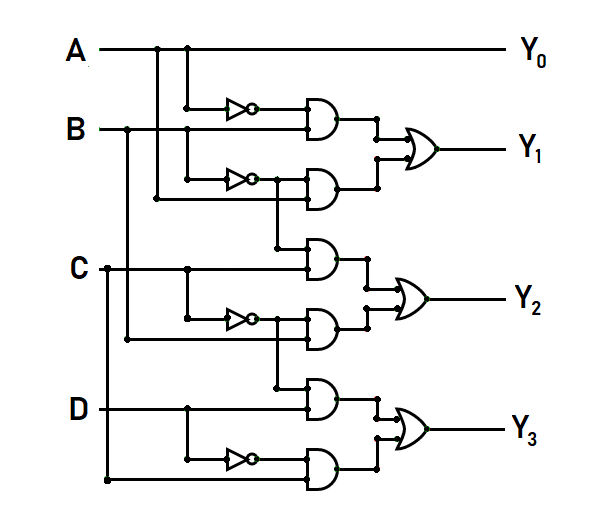
\includegraphics[scale=0.6]{images/logiccircuitej4.png}
    \caption{Representaci\'on de las expresiones mediante un circuito l\'ogico}
    \label{fig:circuito4fig}
\end{figure}

\noindent
El circuito esquematizado en la figura \ref{fig:circuito4fig} es el resultado de expresiones del tipo de suma de productos. Este factor se puede observar en el diagrama debido a que, excepto en $Y_0$ su valor es directamente equivalente al de A, las salidas parten inmediatamente despu\'es de una compuerta OR cuyas entradas siempre son las salidas de dos compuertas AND. 
\subsection{Implementaci\'on en Verilog}
\noindent
En la presente secci\'on se explicita como fue el razonamiento l\'ogico llevado a cabo para la implementaci\'on del circuito en Verilog. Para realizar dicha tarea, se decidi\'o desarrollar un archivo con el m\'odulo principal del circuito y otro archivo con un banco de pruebas.

\noindent
Con respecto al archivo encargado del funcionamiento, lo primero que se realiz\'o fue observar las expresiones de las salidas del circuito para comprender de que manera relacionarlas con la entrada. Al ser 4 entradas y 4 salidas donde cada una representa un nibble, en Verilog se utilizaron arreglos de 4 bits para trabajar sobre ellas. Se define un arreglo como input y luego el otro como output. Por esta raz\'on, se debe tener en cuenta que de las salidas de la convenci\'on utilizada anteriormente, $Y_0$ ser\'a el bit 3 del arreglo de salida y $Y_3$ ser\'a el bit 0.

\noindent
A continuaci\'on, y teniendo en cuenta que $Y_0$ toma el valor de A y que ambos son el bit m\'as significativo de la salida y entrada respectivamente, se igual el bit 3 del arreglo de salida al bit 3 del arreglo de entrada.

\noindent
Como ya fue mencionado, el resto de las salidas pueden ser entendidas como el resultado de una compuerta XOR entre el bit de entrada en la misma posici\'on que el de salida y el de entrada en una posici\'on anterior (m\'as significativo). Este razonamiento se lleva a cabo con las 3 expresiones restantes, siendo estas muy simples al hacer uso de la operaci\'on $'\wedge'$ (XOR) de Verilog. As\'i, por ejemplo, el bit 1 de salida ($Y_2$) depende de un XOR entre el bit 1 y 2 de entrada (B y C).

\noindent
En relaci\'on al banco de pruebas, se utiliz\'o otro archivo .v donde a una entrada de 4 bits se analiza la salida resultante. Este proceso se realiza en el banco para todos los numeros binarios de 4 bits a la entrada y observando si la salida es su correspondiente c\'odigo de Gray. El resultado fue exitoso en todos los casos.
\newpage
\section{Ejercicio 5}

\noindent
El \'ultimo ejercicio requiere la implementaci\'on en Verilog de un m\'odulo multiplicador de dos n\'umeros de un d\'igito en formato BCD, expresando a la salida el resultado como un n\'umero de dos d\'igitos en el mismo formato. \newline
El m\'odulo tiene 3 partes principales: la validaci\'on de la entrada, la multiplicaci\'on en s\'i, y la conversi\'on de binario a BCD del resultado de la multiplicaci\'on. A continuaci\'on se explican consideraciones generales del c\'odigo y las etapas de la implementaci\'on.

\subsection{Consideraciones generales}
\noindent
Se detallan las consideraciones que se tuvieron en cuenta a la hora de programar para lograr una mayor calidad del c\'odigo. 
Hay un m\'odulo principal llamado 'BCDMultiplier', que recibe los n\'umeros BCD a multiplicar en dos arreglos de 4 bits, devuelve el resultado de la multiplicaci\'on en formato BCD en un arreglo de 8 bits, y adem\'as devuelve 2 bits m\'as de validaci\'on que son explicados m\'as adelante.
Todos los arreglos de bits fueron definidos siguiendo la conveci\'on Big Endian ([0:n]), en vez de Little Endian ([n:0]), para tener el bit m\'as significativo en la primera posici\'on, ya que se consider\'o m\'as intuitivo de esa forma. \newline



\subsection{Validaci\'on de la entrada}
\noindent
Antes de proceder a realizar la multiplicaci\'on, es necesario validar que cada nybble recibido corresponda a un n\'umero BCD v\'alido, es decir, que corresponda  a un n\'umero menor a 10. Para poder determinar la validez de un n\'umero recibido, en la Tabla \ref{ej5table} se muestra la tabla de verdad de la validaci\'on, considerando al n\'umero como $X = x_1x_2x_3x_4$ donde se puede observar que la salida toma el valor 1, que se toma como error, si y s\'olo si el valor de la entrada supera el valor de 9, que es el l\'imite para la representaci\'on en un d\'igito BCD.

% Please add the following required packages to your document preamble:
% \usepackage[table,xcdraw]{xcolor}
% If you use beamer only pass "xcolor=table" option, i.e. \documentclass[xcolor=table]{beamer}
\begin{table}[ht]
\centering
\begin{tabular}{|l|c|c|c|c|c|}
\hline
N                        & $x_1$                        & $x_2$                        & $x_3$                        & $x_4$                        & y = $x_1x_2x_3x_4$ \textgreater $b1001$ \\ \hline
0                        & \cellcolor[HTML]{34FF34}0 & \cellcolor[HTML]{34FF34}0 & \cellcolor[HTML]{34FF34}0 & \cellcolor[HTML]{34FF34}0 & \cellcolor[HTML]{FD6864}0          \\ \hline
1                        & \cellcolor[HTML]{34FF34}0 & \cellcolor[HTML]{34FF34}0 & \cellcolor[HTML]{34FF34}0 & \cellcolor[HTML]{34FF34}1 & \cellcolor[HTML]{FD6864}0          \\ \hline
2                        & \cellcolor[HTML]{34FF34}0 & \cellcolor[HTML]{34FF34}0 & \cellcolor[HTML]{34FF34}1 & \cellcolor[HTML]{34FF34}0 & \cellcolor[HTML]{FD6864}0          \\ \hline
3                        & \cellcolor[HTML]{34FF34}0 & \cellcolor[HTML]{34FF34}0 & \cellcolor[HTML]{34FF34}1 & \cellcolor[HTML]{34FF34}1 & \cellcolor[HTML]{FD6864}0          \\ \hline
4                        & \cellcolor[HTML]{34FF34}0 & \cellcolor[HTML]{34FF34}1 & \cellcolor[HTML]{34FF34}0 & \cellcolor[HTML]{34FF34}0 & \cellcolor[HTML]{FD6864}0          \\ \hline
5                        & \cellcolor[HTML]{34FF34}0 & \cellcolor[HTML]{34FF34}1 & \cellcolor[HTML]{34FF34}0 & \cellcolor[HTML]{34FF34}1 & \cellcolor[HTML]{FD6864}0          \\ \hline
6                        & \cellcolor[HTML]{34FF34}0 & \cellcolor[HTML]{34FF34}1 & \cellcolor[HTML]{34FF34}1 & \cellcolor[HTML]{34FF34}0 & \cellcolor[HTML]{FD6864}0          \\ \hline
7                        & \cellcolor[HTML]{34FF34}0 & \cellcolor[HTML]{34FF34}1 & \cellcolor[HTML]{34FF34}1 & \cellcolor[HTML]{34FF34}1 & \cellcolor[HTML]{FD6864}0          \\ \hline
8                        & \cellcolor[HTML]{34FF34}1 & \cellcolor[HTML]{34FF34}0 & \cellcolor[HTML]{34FF34}0 & \cellcolor[HTML]{34FF34}0 & \cellcolor[HTML]{FD6864}0          \\ \hline
9                        & \cellcolor[HTML]{34FF34}1 & \cellcolor[HTML]{34FF34}0 & \cellcolor[HTML]{34FF34}0 & \cellcolor[HTML]{34FF34}1 & \cellcolor[HTML]{FD6864}0          \\ \hline
10                       & \cellcolor[HTML]{34FF34}1 & \cellcolor[HTML]{34FF34}0 & \cellcolor[HTML]{34FF34}1 & \cellcolor[HTML]{34FF34}0 & \cellcolor[HTML]{FD6864}1          \\ \hline
\multicolumn{1}{|c|}{11} & \cellcolor[HTML]{34FF34}1 & \cellcolor[HTML]{34FF34}0 & \cellcolor[HTML]{34FF34}1 & \cellcolor[HTML]{34FF34}1 & \cellcolor[HTML]{FD6864}1          \\ \hline
12                       & \cellcolor[HTML]{34FF34}1 & \cellcolor[HTML]{34FF34}1 & \cellcolor[HTML]{34FF34}0 & \cellcolor[HTML]{34FF34}0 & \cellcolor[HTML]{FD6864}1          \\ \hline
13                       & \cellcolor[HTML]{34FF34}1 & \cellcolor[HTML]{34FF34}1 & \cellcolor[HTML]{34FF34}0 & \cellcolor[HTML]{34FF34}1 & \cellcolor[HTML]{FD6864}1          \\ \hline
14                       & \cellcolor[HTML]{34FF34}1 & \cellcolor[HTML]{34FF34}1 & \cellcolor[HTML]{34FF34}1 & \cellcolor[HTML]{34FF34}0 & \cellcolor[HTML]{FD6864}1          \\ \hline
15                       & \cellcolor[HTML]{34FF34}1 & \cellcolor[HTML]{34FF34}1 & \cellcolor[HTML]{34FF34}1 & \cellcolor[HTML]{34FF34}1 & \cellcolor[HTML]{FD6864}1          \\ \hline

\end{tabular}
\label{ej5table}
\caption{Tabla de verdad de la validaci\'on de la entrada}
\end{table}

\noindent
De la tabla se obtiene el siguiente mapa de Karnaugh:


%Empty Karnaugh map 4x4
\newenvironment{Karnaugh3}%
{
\begin{tikzpicture}[baseline=(current bounding box.north),scale=0.8]
\draw (0,0) grid (4,4);
\draw (0,4) -- node [pos=0.7,above right,anchor=south west] {$x_3x_4$} node [pos=0.7,below left,anchor=north east] {$x_1x_2$} ++(120:1);
%
\matrix (mapa) [matrix of nodes,
        column sep={0.8cm,between origins},
        row sep={0.8cm,between origins},
        every node/.style={minimum size=0.3mm},
        anchor=8.center,
        ampersand replacement=\&] at (0.5,0.5)
{
                       \& |(c00)| 00         \& |(c01)| 01         \& |(c11)| 11         \& |(c10)| 10         \& |(cf)| \phantom{00} \\
|(r00)| 00             \& |(0)|  \phantom{0} \& |(1)|  \phantom{0} \& |(3)|  \phantom{0} \& |(2)|  \phantom{0} \&                     \\
|(r01)| 01             \& |(4)|  \phantom{0} \& |(5)|  \phantom{0} \& |(7)|  \phantom{0} \& |(6)|  \phantom{0} \&                     \\
|(r11)| 11             \& |(12)| \phantom{0} \& |(13)| \phantom{0} \& |(15)| \phantom{0} \& |(14)| \phantom{0} \&                     \\
|(r10)| 10             \& |(8)|  \phantom{0} \& |(9)|  \phantom{0} \& |(11)| \phantom{0} \& |(10)| \phantom{0} \&                     \\
|(rf) | \phantom{00}   \&                    \&                    \&                    \&                    \&                     \\
};
}%
{
\end{tikzpicture}
}

\begin{center}
\begin{Karnaugh3}
    \centering
    \maxterms{0,1,2,3,4,5,6,7,8,9}
    \minterms{10,11,12,13,14,15}
    \implicant{15}{10}{red}
    \implicant{12}{14}{blue}
\end{Karnaugh3}
\end{center}



\noindent
Resolviendo para los mint\'erminos, se llega a la siguiente suma de productos: 
\begin{equation}
    y = x_1\cdot x_2 + x_1\cdot x_3
    \label{ej5_validation_eq}
\end{equation}
\noindent
Por lo tanto, para validar los n\'umeros de entrada, basta implementar la Ecuaci\'on \ref{ej5_validation_eq}. \\
A la hora de la implementaci\'on en Verilog, se decidi\'o realizar un m\'odulo espec\'ifico que realice la validaci\'on, mediante la expresi\'on l\'ogica obtenida anteriormente. Esta validaci\'on se realiza para ambos n\'umeros de entrada, y el m\'odulo principal tiene dos bits de output para indicar la validez de cada par\'ametro de entrada.
\subsection{Multiplicaci\'on binaria y conversi\'on a BCD}
\noindent
Una vez validada la entrada, se debe realizar la multiplicaci\'on en binario. Para esto se hace uso del operador '*' de Verilog, que arroja el resultado de la multiplicaci\'on binaria. Teniendo el resultado en binario de la multiplicaci\'on, hay m\'ultiples formas de pasarlo a BCD. En primer lugar se hab\'ia decidido implementar el algoritmo DoubleDabble, pero la implementaci\'on no era acorde a la filosof\'ia de Verilog, ya que hab\'ia que realizar muchas iteraciones. Dado que realizar una tabla de verdad involucraba m\'as de 50 casos, se utiliz\'o el operador \% (m\'odulo) de Verilog, para obtener las decenas y las unidades.
\subsection{Banco de pruebas}
\noindent
El banco de pruebas prueba 6 casos que se consideran representativos de la totalidad de entradas que puede tener el m\'odulo. En primer lugar, se prueba si una multiplicaci\'on por 0 arroja 0 como resultado. Los siguientes dos casos son multiplicaciones v\'alidas con resultado distinto de 0. Por \'ultimo, hay 3 casos inv\'alidos, en los que se puede observar que el m\'odulo distingue cu\'al de sus entradas es inv\'alida. \\
Para que el c\'odigo del banco de pruebas no fuera repetitivo, se utilizaron tasks de Verilog para las salidas hacia el usuario.
\newpage
\section{Conclusi\'on}
\noindent
A modo de cierre, a lo largo del informe se pudieron desarrollar las tem\'aticas propuestas y cumplir los objetivos planteados.
Fue posible utilizar las herramientas fundamentales de la l\'ogica combinacional, es decir, tablas de verdad y mapas de Karnaugh,
para la implementaci\'on circuital gr\'afica o programada. En cuanto al lenguaje Verilog, se tuvo una primera aproximaci\'on
a los lenguajes de programaci\'on funcionales, mediante la implementaci\'on de m\'odulos. Adicionalmente, se desarrollaron bancos de 
pruebas para verificar el correcto funcionamiento de los m\'odulos. 
Por \'ultimo, para el trabajo fue utilizada la herramienta GitHub, muy utilizada en el \'ambito profesional para llevar un control
de versiones de los avances. 

\end{document}
